\section{Confronto tra modelli}
I quattro modelli addestrati portano tutti a ottime performance, ma i loro 
tempi di addestramento variano notevolmente.
Per scegliere il modello migliore, quindi, vengono analizzati sia il macro-f1 score
sia il tempo di addestramento.

Per calcolare valore medio e intervallo di confidenza di entrambe
le misurazioni, viene eseguita
una stratified cross-validation con 10 fold. Questo numero di fold è stato 
scelto perchè esperimenti passati hanno dimostrato che un tale numero di fold
permette di approssimare bene i valori reali.

Per quanto riguarda il macro-f1 score, tutti i modelli presentano un
valore medio maggiore del $90\%$. In particolare, i valori medi dei quattro modelli
sono: \begin{itemize*}
    \item albero decisionale = $91,1\%$
    \item MLP = $93,2\%$
    \item SVM = $93,8\%$
    \item Gaussian Naive Bayes = $91,5\%$
\end{itemize*}
Gli intervalli di confidenza al $90\%$ del macro-f1 score sono invece:
\begin{itemize*}
    \item albero decisionale = $(90,7\%, 91,4\%)$
    \item MLP = $(92,9\%, 93,5\%)$
    \item SVM = $(93,6\%, 94,1\%)$
    \item Gaussian Naive Bayes = $(91,1\%, 91,8\%)$
\end{itemize*}
Il modello con le performance migliori è, quindi, la SVM.

\begin{Figure}
    \centering
    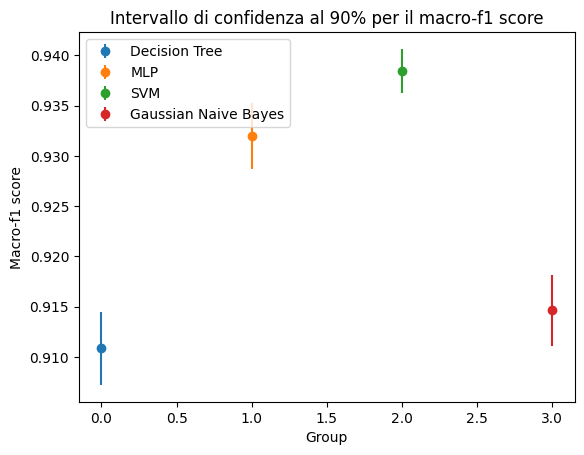
\includegraphics[width=\linewidth]{img/confidence_interval_perf.png}
    \captionof{figure}{Intervallo di confidenza al 90\% per il macro-f1 score.}
\end{Figure}

Analizzando i tempi di addestramento medi, però, si può osservare che
SVM e MLP richiedono molto più tempo per essere addestrate rispetto
agli altri due modelli: \begin{itemize*}
    \item albero decisionale = 88 ms
    \item MLP = 2003 ms
    \item SVM = 987 ms
    \item Gaussian Naive Bayes = 5 ms
\end{itemize*}
L'intervallo di confidenza al $90\%$ del tempo di addestramento è: \begin{itemize*}
    \item albero decisionale = (82 ms, 94 ms)
    \item MLP = (1617 ms, 2389 ms)
    \item SVM = (817 ms, 1156 ms)
    \item Gaussian Naive Bayes = (4 ms, 5 ms)
\end{itemize*}

\textit{NOTA}: i tempi di esecuzione qui riportati non possono essere identici a quelli 
rilevati su Colab. 
Il tempo di esecuzione dipende, infatti, da molti fattori, tra cui il 
carico dei server di Google Colab. Si può affermare, però, che i tempi qui
riportati approssimano bene il tempo di addestramento reale.

\begin{Figure}
    \centering
    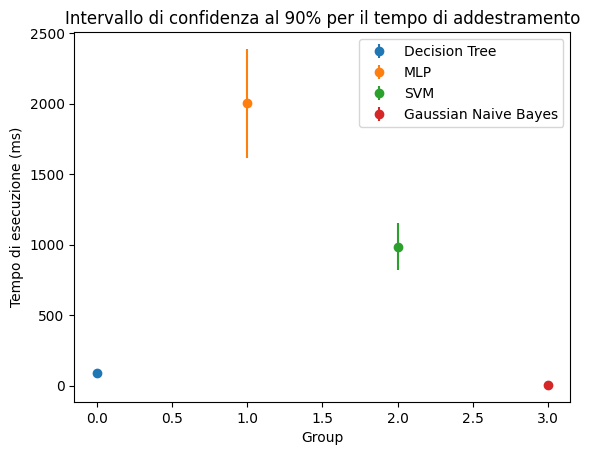
\includegraphics[width=\linewidth]{img/confidence_interval_time.png}
    \captionof{figure}{Intervallo di confidenza al 90\% per il tempo di addestramento.}
\end{Figure}

Tutti i modelli addestrati presentano, quindi, ottime performance.
La scelta del modello migliore, che verrà effettivamente usato 
per la classificazione dei fagioli, ricade principalmente, quindi,
sul tempo di addestramento.
La rete neurale, offrendo prestazioni poco inferiori alla SVM ma con un tempo 
di addestramento maggiore, è il primo modello che è possibile scartare.
Lo stesso ragionamento può essere applicato all'albero decisionale,
in riferimento al Gaussian Naive Bayes classifier.
Tra i due modelli rimanenti, ovvero SVM e Gaussian Naive Bayes, la scelta dipende
dalla tolleranza all'errore che il dominio sopporta: se, infatti,
le performance devono essere massimizzate, allora la scelta ricade sulla SVM, 
e dovranno essere tollerati tempi di addestramento maggiori.
Se, invece, il dominio di applicazione sopporta permormance minori (che in questo
caso sono comunque ottime, in quanto Gaussian Naive Bayes ha un
macro-f1 score medio del $91,5\%$), allora è possibile scegliere Gaussian Naive Bayes,
e beneficiare di tempi di addestramento molto ridotti.

Nel dominio di applicazione considerato in questo progetto, ovvero la classificazione
di fagioli nelle loro varietà, alcuni errori possono essere tollerati, 
in quanto campo a basso impatto d'errore. Di conseguenza, il modello che
sarà mandato in produzione sarà il Gaussian Naive Bayes.